 Define Article %%%%%
\documentclass{article}
%%%%%%%%%%%%%%%%%%%%%

 Using Packages %%%%%
\usepackage{geometry}
\usepackage{graphicx}
\usepackage{amssymb}
\usepackage{amsmath}
\usepackage{amsthm}
\usepackage{empheq}
\usepackage{mdframed}
\usepackage{booktabs}
\usepackage{lipsum}
\usepackage{graphicx}
\usepackage{color}
\usepackage{psfrag}
\usepackage{pgfplots}
\usepackage{bm}
%%%%%%%%%%%%%%%%%%%%%

% Other Settings

%%%%%%%%%%%%%%%%%%%%%%%%%% Page Setting %%%%%%%%%%
\geometry{a4paper}

%%%%%%%%%%%%%%%%%%%%%%%%%% Define some useful colors %%%%%%%%%%%%%%%%%%%%%%%%%%
\definecolor{ocre}{RGB}{243,102,25}
\definecolor{mygray}{RGB}{243,243,244}
\definecolor{deepGreen}{RGB}{26,111,0}
\definecolor{shallowGreen}{RGB}{235,255,255}
\definecolor{deepBlue}{RGB}{61,124,222}
\definecolor{shallowBlue}{RGB}{235,249,255}
%%%%%%%%%%%%%%%%%%%%%

%%%%%%%%%%%%%%%%%%%%%%%%%% Define an orangebox command %%%%%%%%%%%%%%%%%%%%%%%%
\newcommand\orangebox[1]{\fcolorbox{ocre}{mygray}{\hspace{1em}#1\hspace{1em}}}
%%%%%%%%%%%%%%%%%%%%%

%%%%%%%%%%%%%%%%%%%%%%%%%%%% English Environments 
\newtheoremstyle{mytheoremstyle}{3pt}{3pt}{\normalfont}{0cm}{\rmfamily\bfseries}{}{1em}{{\color{black}\thmname{#1}~\thmnumber{#2}}\thmnote{\,--\,#3}}
\newtheoremstyle{myproblemstyle}{3pt}{3pt}{\normalfont}{0cm}{\rmfamily\bfseries}{}{1em}{{\color{black}\thmname{#1}~\thmnumber{#2}}\thmnote{\,--\,#3}}
\theoremstyle{mytheoremstyle}
\newmdtheoremenv[linewidth=1pt,backgroundcolor=shallowGreen,linecolor=deepGreen,leftmargin=0pt,innerleftmargin=20pt,innerrightmargin=20pt,]{theorem}{Theorem}[section]
\theoremstyle{mytheoremstyle}
\newmdtheoremenv[linewidth=1pt,backgroundcolor=shallowBlue,linecolor=deepBlue,leftmargin=0pt,innerleftmargin=20pt,innerrightmargin=20pt,]{definition}{Definition}[section]
\theoremstyle{myproblemstyle}
\newmdtheoremenv[linecolor=black,leftmargin=0pt,innerleftmargin=10pt,innerrightmargin=10pt,]{problem}{Problem}[section]
%%%%%%%%%%%%%%%%%%%%%

%% Plotting Settings 
\usepgfplotslibrary{colorbrewer}
\pgfplotsset{width=8cm,compat=1.9}
%%%%%%%%%%%%%%%%%%%%%

%% Title & Author %%%
\title{Week 3 SEL Activity 3}
\author{Muhammad Meesum Ali Qazalbash}
%%%%%%%%%%%%%%%%%%%%%

\begin{document}
\maketitle\
\begin{equation*}
	\begin{array}{|c|c|c|c|c|c|c|c|c|c|c|c|c|c|c|}
		\hline
		n & 0  & 1  & 2  & 3  & 4  & 5  & 6  & 7  & 8  & 9 & 10 & 11 & 12 & 13+ \\\hline
		F & 14 & 30 & 36 & 68 & 43 & 43 & 30 & 14 & 10 & 6 & 4  & 1  & 1  & 0   \\\hline
	\end{array}
\end{equation*}

Poisson distibution has been used to model the traffic situation. The estimation for \(\lambda\) for observations \(X_1,X_2,X_3,\cdots,X_N\) is given by,
\[\hat{\lambda}=\frac{1}{N}\sum_{i=1}^{N}X_{i}\]
Where \(X_i\) is Poisson random varriable, whose pdf is given by,
\[f_X(n;\lambda)=\begin{cases}
		\displaystyle\frac{\lambda^n e^{-\lambda}}{n!} & n\geq 0 \\
		0                                              & n<0
	\end{cases}\]
We can use the method of moments to estimate the value of \(\lambda\).
\begin{equation*}
	\begin{split}
		\operatorname{E}[X]&=\sum_{n\ge 0}nf_X(n;\lambda)\\
		\operatorname{E}[X]&=\sum_{n\ge 0}n\frac{\lambda^n e^{-\lambda}}{n!}\\
		\operatorname{E}[X]&=e^{-\lambda}\sum_{n\ge 1}\frac{\lambda^n}{(n-1)!}\\
		\operatorname{E}[X]&=e^{-\lambda}\sum_{n\ge 0}\frac{\lambda^{n+1}}{n!}\\
		\operatorname{E}[X]&=\lambda e^{-\lambda}\sum_{n\ge 0}\frac{\lambda^n}{n!}\\
		\operatorname{E}[X]&=\lambda e^{-\lambda}e^{\lambda}\\
		\operatorname{E}[X]&=\lambda
	\end{split}
\end{equation*}
Our first moment is the function of the variable we want to estimate. This mean the estimation of \(\lambda\) will be,
\begin{equation*}
	\begin{split}
		\hat{\lambda}&=\hat{\mu}_1\\
		\hat{\lambda}&=\frac{
			(0)(14)
			+(1)(30)
			+(2)(36)
			+\cdots
			+(11)(1)
			+(12)(1)
			+(13)(0)
		}{300}\\
		\hat{\lambda}&=3.893
	\end{split}
\end{equation*}
The values for \(\hat{\lambda}\) are,
\begin{equation*}
	\begin{array}{|c|c|c|c|c|c|c|c|c|c|c|c|c|c|c|}
		\hline
		n       & 0    & 1     & 2     & 3     & 4     & 5     & 6     & 7     & 8   & 9    & 10   & 11   & 12   & 13+  \\\hline
		\hat{F} & 6.12 & 23.81 & 46.34 & 60.13 & 58.52 & 45.57 & 29.57 & 16.44 & 8.0 & 3.46 & 1.35 & 0.48 & 0.15 & 0.05 \\\hline
	\end{array}
\end{equation*}
\begin{figure}[h]
	\center
	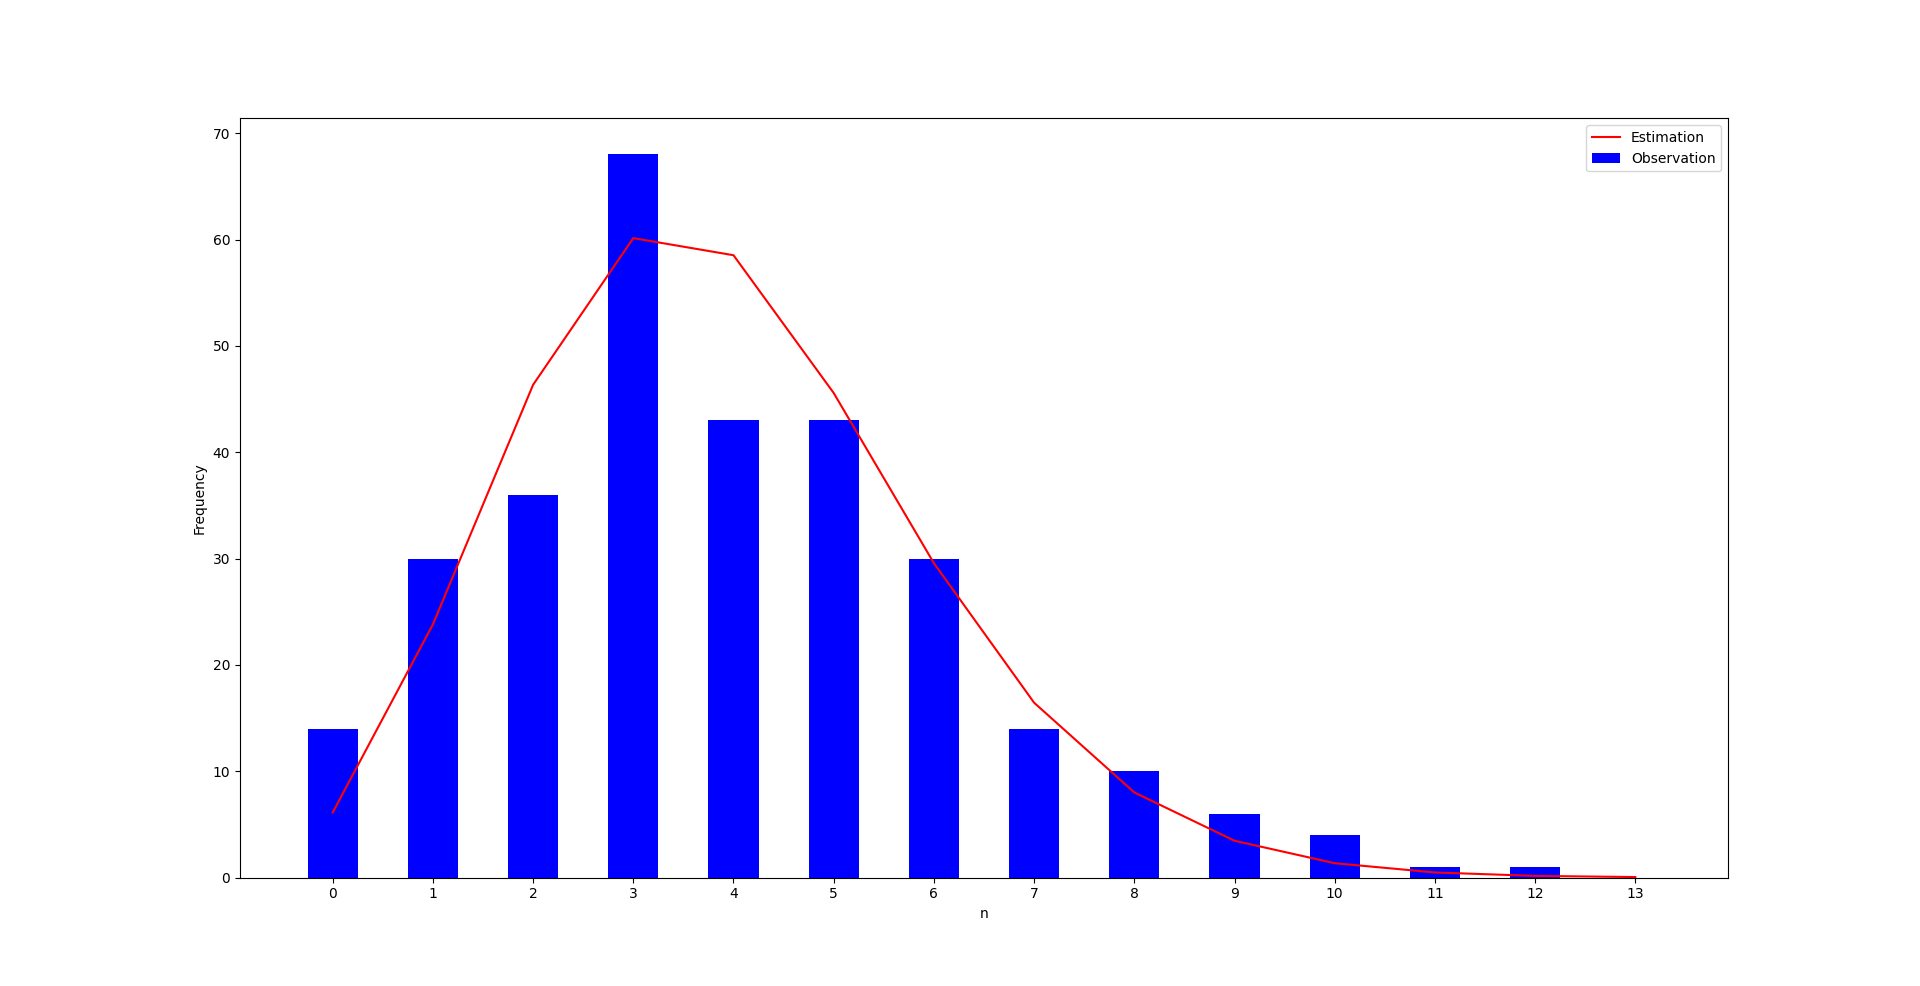
\includegraphics[width=\textwidth]{fig.png}
\end{figure}

As most of the values are in the vicinity of 3 and 4 and around those values our estimator is not estimating good. Hence we made a bad estimator.
\end{document}